\documentclass[tikz,border=20pt]{standalone}
\usepackage{tikz}
\usetikzlibrary{shapes, arrows.meta, positioning, fit, backgrounds, calc, shadows}
\definecolor{acaBlueLine}{HTML}{6080B0}      \definecolor{acaBlueFill}{HTML}{DBEAFE}
\definecolor{acaGreenLine}{HTML}{30A060}     \definecolor{acaGreenFill}{HTML}{A0D0A0}
\definecolor{acaOrangeLine}{HTML}{D06020}    \definecolor{acaOrangeFill}{HTML}{FFE6CC}
\definecolor{acaPurpleLine}{HTML}{6020D0}    \definecolor{acaPurpleFill}{HTML}{E1D5E7}
\definecolor{zoneGreenBg}{HTML}{ECFDF5}
\definecolor{zoneOrangeBg}{HTML}{FFF5EB}
\pgfdeclarelayer{background}
\pgfsetlayers{background,main}
\begin{document}
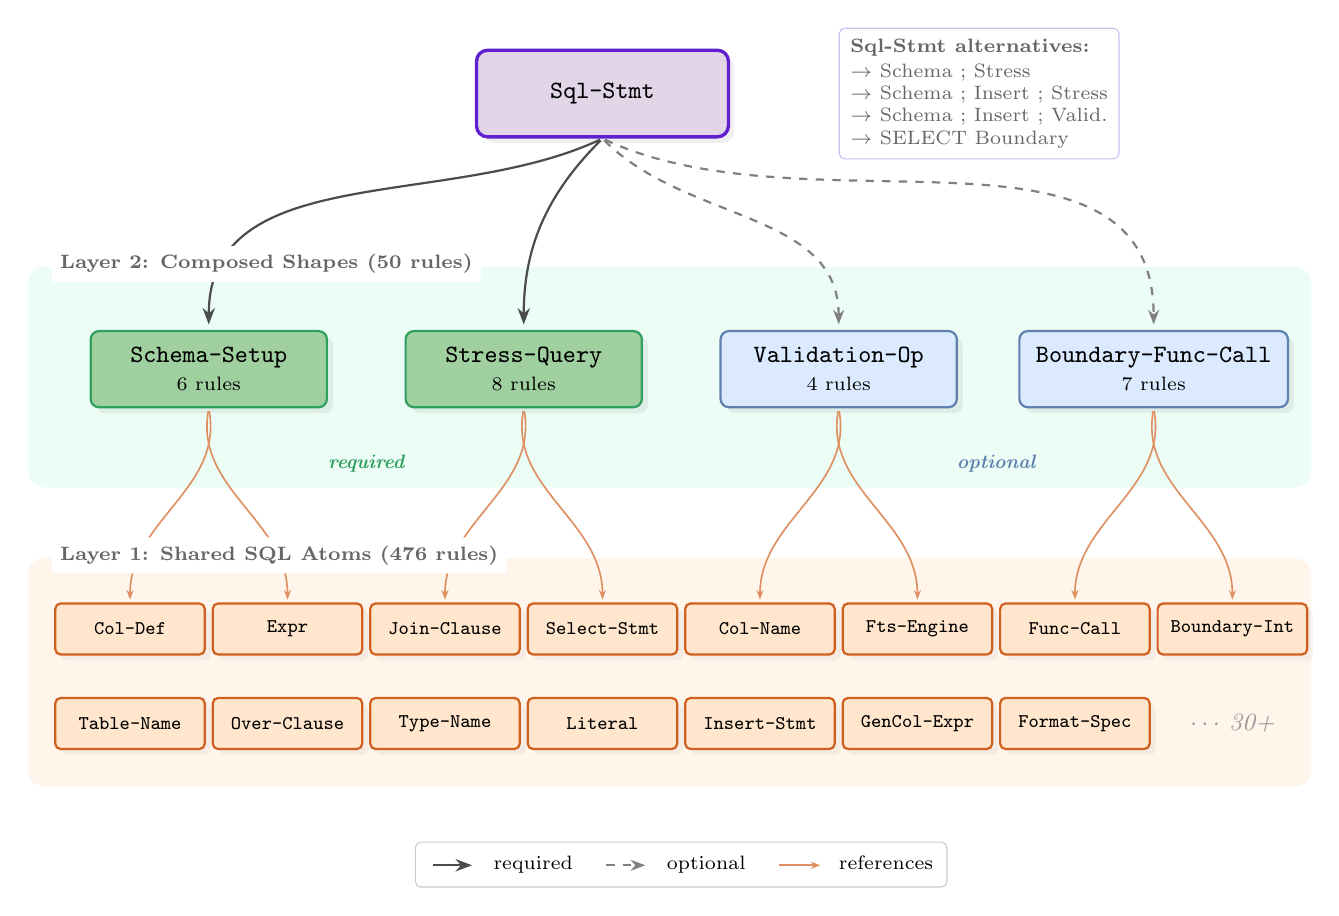
\begin{tikzpicture}[
    every node/.style={font=\small},
    rootbox/.style={rectangle, rounded corners=4pt, align=center,
        minimum width=3.2cm, minimum height=1.1cm,
        inner sep=8pt, very thick, draw=acaPurpleLine, fill=acaPurpleFill,
        drop shadow={opacity=0.12}, font=\small\bfseries},
    l2box/.style={rectangle, rounded corners=3pt, align=center,
        minimum width=3.0cm, minimum height=0.9cm,
        inner sep=6pt, thick, drop shadow={opacity=0.12}},
    l1box/.style={rectangle, rounded corners=2pt, align=center,
        minimum width=1.9cm, minimum height=0.65cm,
        inner sep=4pt, thick, font=\scriptsize,
        drop shadow={opacity=0.08}},
    arrow/.style={-{Stealth[scale=0.9]}, thick, color=black!70,
        shorten >=2pt, shorten <=1pt},
    dasharr/.style={-{Stealth[scale=0.8]}, thick, dashed, color=black!50,
        shorten >=2pt, shorten <=1pt},
    refarr/.style={-{Stealth[scale=0.6]}, semithick, color=acaOrangeLine!70,
        shorten >=1pt, shorten <=1pt},
    zonetag/.style={font=\scriptsize\bfseries, color=black!60,
        fill=white, inner sep=3pt, rounded corners=1pt},
]
    % ═══════════════════════════════════════════
    % ROW 1: Sql-Stmt
    % ═══════════════════════════════════════════
    \node[rootbox] (root) at (7.5, 11) {\texttt{Sql-Stmt}};

    \node[font=\scriptsize, color=black!60, align=left,
          draw=acaPurpleLine!30, rounded corners=2pt, fill=white,
          inner sep=4pt, anchor=west]
        at (10.5, 11) {
        \textbf{\scriptsize Sql-Stmt alternatives:}\\[1pt]
        $\to$ Schema ; Stress\\
        $\to$ Schema ; Insert ; Stress\\
        $\to$ Schema ; Insert ; Valid.\\
        $\to$ SELECT Boundary
    };

    % ═══════════════════════════════════════════
    % ROW 2: Layer 2 — four shapes
    % Each centered over its pair of L1 atoms
    % Pairs at x: (1.5, 3.5), (5.5, 7.5), (9.5, 11.5), (13.5, 15.5)
    % L2 centers: 2.5, 6.5, 10.5, 14.5
    % ═══════════════════════════════════════════
    \node[l2box, fill=acaGreenFill, draw=acaGreenLine] (schema) at (2.5, 7.5) {
        \textbf{\texttt{Schema-Setup}}\\[-1pt]
        {\scriptsize 6 rules}
    };
    \node[l2box, fill=acaGreenFill, draw=acaGreenLine] (stress) at (6.5, 7.5) {
        \textbf{\texttt{Stress-Query}}\\[-1pt]
        {\scriptsize 8 rules}
    };
    \node[l2box, fill=acaBlueFill, draw=acaBlueLine] (valid) at (10.5, 7.5) {
        \textbf{\texttt{Validation-Op}}\\[-1pt]
        {\scriptsize 4 rules}
    };
    \node[l2box, fill=acaBlueFill, draw=acaBlueLine] (boundary) at (14.5, 7.5) {
        \textbf{\texttt{Boundary-Func-Call}}\\[-1pt]
        {\scriptsize 7 rules}
    };

    % Required / Optional labels below L2 boxes
    \node[font=\scriptsize\bfseries\itshape, color=acaGreenLine]
        at (4.5, 6.3) {required};
    \node[font=\scriptsize\bfseries\itshape, color=acaBlueLine]
        at (12.5, 6.3) {optional};

    % ═══════════════════════════════════════════
    % ROW 3: Layer 1 — Shared Pool
    % First row: 2 atoms per L2, side by side directly below
    % Second row: additional shared atoms
    % ═══════════════════════════════════════════
    % Pair under Schema-Setup (center 2.5)
    \node[l1box, fill=acaOrangeFill, draw=acaOrangeLine] (coldef) at (1.5, 4.2) {\texttt{Col-Def}};
    \node[l1box, fill=acaOrangeFill, draw=acaOrangeLine] (expr1)  at (3.5, 4.2) {\texttt{Expr}};
    % Pair under Stress-Query (center 6.5)
    \node[l1box, fill=acaOrangeFill, draw=acaOrangeLine] (joinc)    at (5.5, 4.2) {\texttt{Join-Clause}};
    \node[l1box, fill=acaOrangeFill, draw=acaOrangeLine] (selectst) at (7.5, 4.2) {\texttt{Select-Stmt}};
    % Pair under Validation-Op (center 10.5)
    \node[l1box, fill=acaOrangeFill, draw=acaOrangeLine] (colname) at (9.5, 4.2)  {\texttt{Col-Name}};
    \node[l1box, fill=acaOrangeFill, draw=acaOrangeLine] (ftseng)  at (11.5, 4.2) {\texttt{Fts-Engine}};
    % Pair under Boundary-Func-Call (center 14.5)
    \node[l1box, fill=acaOrangeFill, draw=acaOrangeLine] (funccall) at (13.5, 4.2) {\texttt{Func-Call}};
    \node[l1box, fill=acaOrangeFill, draw=acaOrangeLine] (boundint) at (15.5, 4.2) {\texttt{Boundary-Int}};

    % Second row — additional shared atoms
    \node[l1box, fill=acaOrangeFill, draw=acaOrangeLine] at (1.5, 3.0)  {\texttt{Table-Name}};
    \node[l1box, fill=acaOrangeFill, draw=acaOrangeLine] at (3.5, 3.0)  {\texttt{Over-Clause}};
    \node[l1box, fill=acaOrangeFill, draw=acaOrangeLine] at (5.5, 3.0)  {\texttt{Type-Name}};
    \node[l1box, fill=acaOrangeFill, draw=acaOrangeLine] at (7.5, 3.0)  {\texttt{Literal}};
    \node[l1box, fill=acaOrangeFill, draw=acaOrangeLine] at (9.5, 3.0)  {\texttt{Insert-Stmt}};
    \node[l1box, fill=acaOrangeFill, draw=acaOrangeLine] at (11.5, 3.0) {\texttt{GenCol-Expr}};
    \node[l1box, fill=acaOrangeFill, draw=acaOrangeLine] at (13.5, 3.0) {\texttt{Format-Spec}};
    \node[font=\small\itshape, color=black!40]            at (15.5, 3.0) {$\cdots$ 30+};

    % ═══════════════════════════════════════════
    % ARROWS: Root → Layer 2 (fan out from bottom)
    % ═══════════════════════════════════════════
    \draw[arrow]   (root.south) to[out=-155, in=90] (schema.north);
    \draw[arrow]   (root.south) to[out=-135, in=90] (stress.north);
    \draw[dasharr] (root.south) to[out=-45,  in=90] (valid.north);
    \draw[dasharr] (root.south) to[out=-25,  in=90] (boundary.north);

    % ═══════════════════════════════════════════
    % ARROWS: Layer 2 → Layer 1 (2 per shape, slight fan)
    % ═══════════════════════════════════════════
    \draw[refarr] (schema.south)   to[out=-80,  in=90] (coldef.north);
    \draw[refarr] (schema.south)   to[out=-100, in=90] (expr1.north);

    \draw[refarr] (stress.south)   to[out=-80,  in=90] (joinc.north);
    \draw[refarr] (stress.south)   to[out=-100, in=90] (selectst.north);

    \draw[refarr] (valid.south)    to[out=-80,  in=90] (colname.north);
    \draw[refarr] (valid.south)    to[out=-100, in=90] (ftseng.north);

    \draw[refarr] (boundary.south) to[out=-80,  in=90] (funccall.north);
    \draw[refarr] (boundary.south) to[out=-100, in=90] (boundint.north);

    % ═══════════════════════════════════════════
    % ZONE BACKGROUNDS
    % ═══════════════════════════════════════════
    \begin{pgfonlayer}{background}
        \fill[zoneGreenBg, rounded corners=6pt]
            (0.2, 6.0) rectangle (16.5, 8.8);
        \fill[zoneOrangeBg, rounded corners=6pt]
            (0.2, 2.2) rectangle (16.5, 5.1);
    \end{pgfonlayer}

    % Zone titles — placed on the zone border so arrows don't cross them
    \node[zonetag, anchor=south west] at (0.5, 8.6) {Layer 2: Composed Shapes (50 rules)};
    \node[zonetag, anchor=south west] at (0.5, 4.9) {Layer 1: Shared SQL Atoms (476 rules)};

    % ═══════════════════════════════════════════
    % LEGEND
    % ═══════════════════════════════════════════
    \node[font=\scriptsize, anchor=north,
          draw=black!20, rounded corners=2pt, fill=white, inner sep=5pt]
        at (8.5, 1.5) {
        \tikz[baseline=-0.5ex] \draw[arrow] (0,0) -- (0.6,0);
        ~required \quad
        \tikz[baseline=-0.5ex] \draw[dasharr] (0,0) -- (0.6,0);
        ~optional \quad
        \tikz[baseline=-0.5ex] \draw[refarr] (0,0) -- (0.6,0);
        ~references
    };
\end{tikzpicture}
\end{document}
